\begin{figure}
    \caption{Recursive quadrant encoding of an $8 \times 8$ DDT. Item (a) shows the whole table divided into 4 quadrants; Item (b) shows each quadrant further divided into 4 subquadrants; Item (c) highlights the cell encoded as \texttt{320}.}
    \label{fig:encoding_example}

    \centering

    \vspace{1em}

    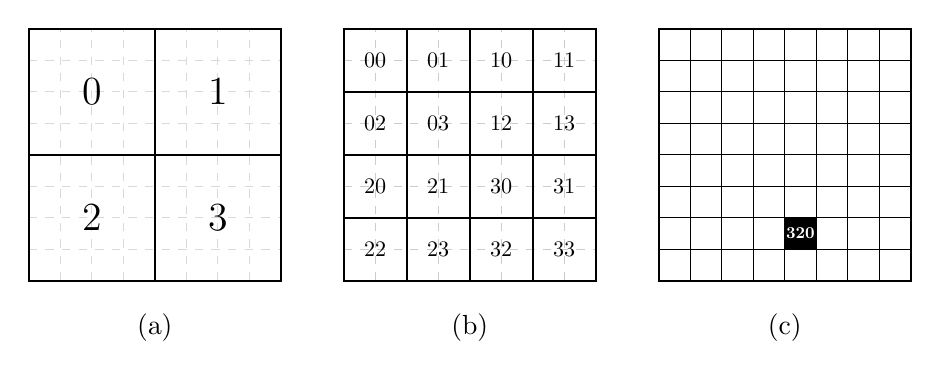
\begin{tikzpicture}[scale=0.4]
        \begin{scope}[shift={(0,0)}]
            \draw[step=1, gray!30, thin, dashed] (0,0) grid (8,8);
            \draw[thick] (0,0) rectangle (8,8);
            \draw[thick] (4,0) -- (4,8);
            \draw[thick] (0,4) -- (8,4);
            
            \node at (2,6) {\Large 0};
            \node at (6,6) {\Large 1};
            \node at (2,2) {\Large 2};
            \node at (6,2) {\Large 3};
            \node at (4,-1.5) {\normalsize (a)};
        \end{scope}

        \begin{scope}[shift={(10,0)}]
            \draw[step=1, gray!40, thin, dashed] (0,0) grid (8,8);
            \draw[thick] (0,0) rectangle (8,8);
            \draw[thick] (4,0) -- (4,8);
            \draw[thick] (0,4) -- (8,4);
            \draw[thick] (2,0) -- (2,8); \draw[thick] (6,0) -- (6,8);
            \draw[thick] (0,2) -- (8,2); \draw[thick] (0,6) -- (8,6);

            \foreach \x/\y/\label in {1/7/00, 3/7/01, 1/5/02, 3/5/03, 5/7/10, 7/7/11, 5/5/12, 7/5/13, 1/3/20, 3/3/21, 1/1/22, 3/1/23, 5/3/30, 7/3/31, 5/1/32, 7/1/33} {
                \node[scale=0.8] at (\x,\y) {\normalsize \label};
            }
            \node at (4,-1.5) {\normalsize (b)};
        \end{scope}

        \begin{scope}[shift={(20,0)}]
            \draw[step=1, thin] (0,0) grid (8,8);
            \draw[thick] (0,0) rectangle (8,8);
            
            \fill[black] (4,1) rectangle (5,2); 
            \node[scale=0.6, text=white, font=\bfseries] at (4.5,1.5) {320};
            \node at (4,-1.5) {\normalsize (c)};
        \end{scope}
    \end{tikzpicture}
\end{figure}






% \begin{table}[ht]
%     \caption{Recursive quadrant encoding representations.}
%     \label{tab:encoding_example}
%     \centering
%     \renewcommand{\arraystretch}{1.0}
%     \setlength{\tabcolsep}{4pt}
%     \begin{tabular}{c@{\hskip 0.3in}c@{\hskip 0.3in}c}
%         \begin{tabular}{|*{8}{c|}}
%         \hline
%         ~ & ~ & ~ & ~ & ~ & ~ & ~ & ~ \\ \hline
%         ~ & ~ & ~ & ~ & ~ & ~ & ~ & ~ \\ \hline
%         ~ & ~ & ~ & ~ & ~ & ~ & ~ & ~ \\ \hline
%         ~ & ~ & ~ & ~ & ~ & ~ & ~ & ~ \\ \hline
%         ~ & ~ & ~ & ~ & ~ & ~ & ~ & ~ \\ \hline
%         ~ & ~ & ~ & ~ & ~ & ~ & ~ & ~ \\ \hline
%         ~ & ~ & ~ & ~ & ~ & ~ & ~ & ~ \\ \hline
%         ~ & ~ & ~ & ~ & ~ & ~ & ~ & ~ \\ \hline
%         \end{tabular}
%         &
%         \begin{tabular}{|*{8}{c|}}
%         \hline
%         ~ & ~ & ~ & ~ & ~ & ~ & ~ & ~ \\ \hline
%         ~ & ~ & ~ & ~ & ~ & ~ & ~ & ~ \\ \hline
%         ~ & ~ & ~ & ~ & ~ & ~ & ~ & ~ \\ \hline
%         ~ & ~ & ~ & ~ & ~ & ~ & ~ & ~ \\ \hline
%         ~ & ~ & ~ & ~ & ~ & ~ & ~ & ~ \\ \hline
%         ~ & ~ & ~ & ~ & ~ & ~ & ~ & ~ \\ \hline
%         ~ & ~ & ~ & ~ & ~ & ~ & ~ & ~ \\ \hline
%         ~ & ~ & ~ & ~ & ~ & ~ & ~ & ~ \\ \hline
%         \end{tabular}
%         &
%         \begin{tabular}{|*{8}{c|}}
%         \hline
%         ~ & ~ & ~ & ~ & ~ & ~ & ~ & ~ \\ \hline
%         ~ & ~ & ~ & ~ & ~ & ~ & ~ & ~ \\ \hline
%         ~ & ~ & ~ & ~ & ~ & ~ & ~ & ~ \\ \hline
%         ~ & ~ & ~ & ~ & ~ & ~ & ~ & ~ \\ \hline
%         ~ & ~ & ~ & ~ & ~ & ~ & ~ & ~ \\ \hline
%         ~ & ~ & ~ & ~ & ~ & ~ & ~ & ~ \\ \hline
%         ~ & ~ & ~ & ~ & ~ & ~ & ~ & ~ \\ \hline
%         ~ & ~ & ~ & ~ & ~ & ~ & ~ & ~ \\ \hline
%         \end{tabular} \\
%         (a) & (b) & (c)
%     \end{tabular}
% \end{table}



% \begin{table}
%     \caption{Recursive quadrant encoding for a $8 \times 8$ DDT. Each cell is uniquely identified by a 4-symbol word. For example, the highlighted region corresponds to all words with the prefix \texttt{320}.}
%     \label{tab:encoding_example}
    
%     \centering
%     \renewcommand{\arraystretch}{1.4}
%     \ttfamily
    
%     \begin{tabular}{|*{16}{C{0.08\textwidth}|}}
    
%     \hline

%     \multicolumn{8}{|C{0.32\textwidth}|}{\multirow{8}{*}{\Huge 0}} & \multicolumn{4}{C{0.16\textwidth}|}{\multirow{4}{*}{\Large 10}} & \multicolumn{4}{C{0.16\textwidth}|}{\multirow{4}{*}{\Large 11}} \\
%     \multicolumn{8}{|C{0.08\textwidth}|}{}                         & \multicolumn{4}{C{0.08\textwidth}|}{}                           & \multicolumn{4}{C{0.08\textwidth}|}{}                           \\
%     \multicolumn{8}{|C{0.08\textwidth}|}{}                         & \multicolumn{4}{C{0.08\textwidth}|}{}                           & \multicolumn{4}{C{0.08\textwidth}|}{}                           \\
%     \multicolumn{8}{|C{0.08\textwidth}|}{}                         & \multicolumn{4}{C{0.08\textwidth}|}{}                           & \multicolumn{4}{C{0.08\textwidth}|}{}                           \\
    
%     \cline{9-16}
    
%     \multicolumn{8}{|C{0.08\textwidth}|}{}                         & \multicolumn{4}{C{0.16\textwidth}|}{\multirow{4}{*}{\Large 12}} & \multicolumn{4}{C{0.16\textwidth}|}{\multirow{4}{*}{\Large 13}} \\
%     \multicolumn{8}{|C{0.08\textwidth}|}{}                         & \multicolumn{4}{C{0.08\textwidth}|}{}                           & \multicolumn{4}{C{0.08\textwidth}|}{}                           \\
%     \multicolumn{8}{|C{0.08\textwidth}|}{}                         & \multicolumn{4}{C{0.08\textwidth}|}{}                           & \multicolumn{4}{C{0.08\textwidth}|}{}                           \\
%     \multicolumn{8}{|C{0.08\textwidth}|}{}                         & \multicolumn{4}{C{0.08\textwidth}|}{}                           & \multicolumn{4}{C{0.08\textwidth}|}{}                           \\
    
%     \hline
    
%     \multicolumn{2}{|C{0.08\textwidth}|}{\multirow{2}{*}{200}} & \multicolumn{2}{C{0.08\textwidth}|}{\multirow{2}{*}{201}} & \multicolumn{2}{C{0.08\textwidth}|}{\multirow{2}{*}{210}} & \multicolumn{2}{C{0.08\textwidth}|}{\multirow{2}{*}{211}} & \multicolumn{2}{C{0.08\textwidth}|}{\multirow{2}{*}{300}}  & \multicolumn{2}{C{0.08\textwidth}|}{\multirow{2}{*}{301}} & \multicolumn{2}{C{0.08\textwidth}|}{\multirow{2}{*}{310}} & \multicolumn{2}{C{0.08\textwidth}|}{\multirow{2}{*}{311}} \\
    
%     \multicolumn{2}{|C{0.08\textwidth}|}{}                     & \multicolumn{2}{C{0.08\textwidth}|}{}                     & \multicolumn{2}{C{0.08\textwidth}|}{}                     & \multicolumn{2}{C{0.08\textwidth}|}{}                     & \multicolumn{2}{C{0.08\textwidth}|}{}                      & \multicolumn{2}{C{0.08\textwidth}|}{}                     & \multicolumn{2}{C{0.08\textwidth}|}{}                         & \multicolumn{2}{C{0.08\textwidth}|}{}                     \\ 
    
%     \cline{1-16}
    
%     % Row 11-12: Sub-quadrants 20 and 21 (left), 30 and 31 (right)
%     \multicolumn{2}{|C{0.08\textwidth}|}{\multirow{2}{*}{202}} & \multicolumn{2}{C{0.08\textwidth}|}{\multirow{2}{*}{203}} & \multicolumn{2}{C{0.08\textwidth}|}{\multirow{2}{*}{212}} & \multicolumn{2}{C{0.08\textwidth}|}{\multirow{2}{*}{213}} & \multicolumn{2}{C{0.08\textwidth}|}{\multirow{2}{*}{302}}  & \multicolumn{2}{C{0.08\textwidth}|}{\multirow{2}{*}{303}} & \multicolumn{2}{C{0.08\textwidth}|}{\multirow{2}{*}{312}} & \multicolumn{2}{C{0.08\textwidth}|}{\multirow{2}{*}{313}} \\
    
%     \multicolumn{2}{|C{0.08\textwidth}|}{}                     & \multicolumn{2}{C{0.08\textwidth}|}{}                     & \multicolumn{2}{C{0.08\textwidth}|}{}                     & \multicolumn{2}{C{0.08\textwidth}|}{}                     & \multicolumn{2}{C{0.08\textwidth}|}{}                      & \multicolumn{2}{C{0.08\textwidth}|}{}                     & \multicolumn{2}{C{0.08\textwidth}|}{}                         & \multicolumn{2}{C{0.08\textwidth}|}{}                     \\
    
%     \hline
    
%     % Row 13-14: Sub-quadrants 22 and 23 (left), 32 and 33 (right)
%     \multicolumn{2}{|C{0.08\textwidth}|}{\multirow{2}{*}{220}}  & \multicolumn{2}{C{0.08\textwidth}|}{\multirow{2}{*}{221}} & \multicolumn{2}{C{0.08\textwidth}|}{\multirow{2}{*}{230}} & \multicolumn{2}{C{0.08\textwidth}|}{\multirow{2}{*}{231}} & \multicolumn{2}{C{0.08\textwidth}|}{\cellcolor{Color1}\multirow{2}{*}{320}} & \multicolumn{2}{C{0.08\textwidth}|}{\multirow{2}{*}{321}} & \multicolumn{2}{C{0.08\textwidth}|}{\multirow{2}{*}{330}} & \multicolumn{2}{C{0.08\textwidth}|}{\multirow{2}{*}{331}} \\
    
%     \multicolumn{2}{|C{0.08\textwidth}|}{}                      & \multicolumn{2}{C{0.08\textwidth}|}{}                     & \multicolumn{2}{C{0.08\textwidth}|}{}                     & \multicolumn{2}{C{0.08\textwidth}|}{}                     & \multicolumn{2}{C{0.08\textwidth}|}{\cellcolor{Color1}\multirow{-2}{*}{320}}                     & \multicolumn{2}{C{0.08\textwidth}|}{}                     & \multicolumn{2}{C{0.08\textwidth}|}{}                     & \multicolumn{2}{C{0.08\textwidth}|}{}                     \\
    
%     \cline{1-16}
    
%     % Row 15-16: Sub-quadrants 22 and 23 (left), 32 and 33 (right)
%     \multicolumn{2}{|C{0.08\textwidth}|}{\multirow{2}{*}{222}} & \multicolumn{2}{C{0.08\textwidth}|}{\multirow{2}{*}{223}} & \multicolumn{2}{C{0.08\textwidth}|}{\multirow{2}{*}{232}} & \multicolumn{2}{C{0.08\textwidth}|}{\multirow{2}{*}{233}} & \multicolumn{2}{C{0.08\textwidth}|}{\multirow{2}{*}{322}} & \multicolumn{2}{C{0.08\textwidth}|}{\multirow{2}{*}{323}} & \multicolumn{2}{C{0.08\textwidth}|}{\multirow{2}{*}{332}} & \multicolumn{2}{C{0.08\textwidth}|}{\multirow{2}{*}{333}} \\
    
%     \multicolumn{2}{|C{0.08\textwidth}|}{}                     & \multicolumn{2}{C{0.08\textwidth}|}{}                     & \multicolumn{2}{C{0.08\textwidth}|}{}                     & \multicolumn{2}{C{0.08\textwidth}|}{}                     & \multicolumn{2}{C{0.08\textwidth}|}{}                     & \multicolumn{2}{C{0.08\textwidth}|}{}                     & \multicolumn{2}{C{0.08\textwidth}|}{}                          & \multicolumn{2}{C{0.08\textwidth}|}{}                     \\
    
%     \hline
    
%     \end{tabular}
% \end{table}
